\chapter{Caminatas cuánticas sobre gráficas}
Una generalización natural a las caminatas sobre la línea consiste en considerar los vértices de un grafo como las posiciones posibles de la partícula, y los arcos como los posibles caminos. En un vértice $v$ de grado $d$, usamos una moneda de dimensión $d$ para decidir el  camino de traslación. Los estados son $\left\{\ket{j}\otimes\ket{v}|j=0,\dots,d(v);v=0,\dots,|V(\Gamma)| \right\}$. De esta forma hemos definido la evolución desde cada vértice según su grado (evolución \textit{local}), $\hat{U}_v=\hat{S}_v(\hat{C}_v\otimes I)$. Si queremos una evolución \textit{global} de la forma $\hat{U}=\hat{S}(\hat{C}\otimes I)$, siempre tenemos la opción de hacer regular el grafo añadiendo lazos a los vértices de menor grado hasta completarla dimensión $d$. De esta manera se puede factorizar $\hat{C}_v$ de la evolución de cada vértice y expresar la evolución global de la forma $\hat{U}=\hat{S}(\hat{C}\otimes I)$. Entonces el nuevo espacio es $\mathcal{H}=\mathcal{H}_C\otimes\mathcal{H}_P$.\\

La nueva moneda de dimensión $d$, $C_d$ es unitaria y tiene más grados de libertad que la de la línea. Casos especiales son las monedas DFT, Hadamard y Grover. La DFT\footnote{es el operador transformada de fourier discreta} es un ejemplo natural de las monedas balanceadas

\begin{equation*}
DFT=\frac{1}{\sqrt{d}}
\begin{pmatrix}
1 & 1 & 1 & \cdots & 1\\
1 & \omega & b & \cdots & \omega^{(d-1)}\\
 &  &\vdots & \cdots & \\
1 & \omega^{(d-1)}  & \omega^{2(d-1)} & \cdots & \omega^{(d-1)(d-1)}
\end{pmatrix},
\end{equation*}{}
donde $\omega=\exp{(i2\pi/d)}$ es la raíz de orden $d$ de la unidad. Al final del lanzamiento la probabilidad igual para cada dirección: $(1/d)$. Para $d=2$, se obtiene el operador de Hadamard.\\


\begin{figure}[ht]
\centering
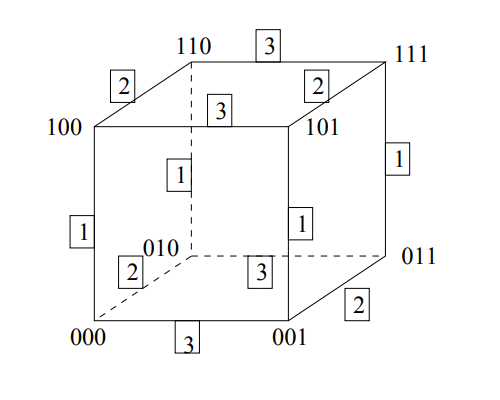
\includegraphics[width=0.8\textwidth]{Kap4/HypercubeKempe.png}
\caption{Hipercubo de dimensión $3$ con etiquetas sobre las aristas.}
\end{figure}

La siguiente moneda no es balanceada pero tiene la propiedad de ser simétrica bajo permutaciones de etiquetas. Esto sucede cuando el grafo es tal que las aristas se pueden etiquetar con el mismo nombre vista desde los dos vértices. El hipercubo es un ejemplo claro de ello.

\begin{equation*}
G_{a,b}\doteq
\begin{pmatrix}
a & b & b & \cdots & b\\
b & a & b & \cdots & b\\
 & \vdots & & \ddots & \\
b & b  & b & \cdots & a
\end{pmatrix}
\end{equation*}{}
con $1-\frac{2}{d}\leq|a|\leq 1$, y $b=\pm(1-a)$. Cuando $a=\frac{2}{d}-1$, $b=$ la moneda es la más se aleja de la identidad, $G_{0,1}=\mathbb{I}$, y se llama operador de Grover. \\

Con el producto tensorial de dos monedas de Hadamard obtenemos $\hat{H}^{\otimes 2}$ de grado 4. En general, podemos hacer monedas de orden $2^n$ a partir de $\hat{H}$: $\hat{H}^{\otimes n}$.

\section{El plano infinito}
A continuación se muestran las caminatas sobre el plano infinito construido con una red cuadrada para las monedas de Hadamard, Grover y Fourier. 

\subsubsection*{Grover}
\begin{equation}
H=\frac{1}{2}
\begin{pmatrix}
-1 & 1 & 1 & 1\\
1 & -1 & 1 & 1\\
1 & 1 & -1 & 1\\
1 & 1 & 1 & -1
\end{pmatrix}
\qquad ; \qquad    \ket{\Psi(0)}=\frac{1}{2}(\ket{00}-\ket{01}-\ket{10}+\ket{11})\otimes\ket{x=0,y=0}
\end{equation}{}

\begin{figure}[ht]
\caption{}
\centering
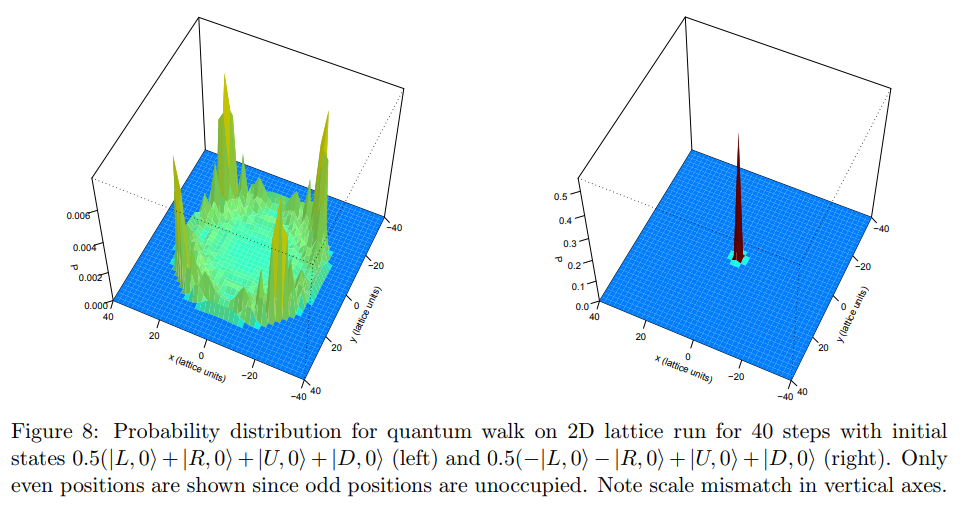
\includegraphics[width=0.9\textwidth]{Kap4/QWGroverCoinKendonPercolation2019.png}
\end{figure}

\section{Dinámica}
En el análisis de la dinámica definimos el \textit{periodo} y \textit{cuasi-periodo} de la distribución y mostramos que la unitariedad del proceso conserva la información de la condición inicial, y no es posible converger en una distribución límite, a diferencia del caso clásico. Sin embargo, es común usar una distribución uniforme sobre las distribuciones originales con distintas condiciones iniciales que elimina la 'memoria' de los estados iniciales en el sistema permitiendo alcanzar una distribución estacionaria límite sobre esta nueva distribución. Introducimos los conceptos de \textit{mixing time} y \textit{hitting time} que destacan diferencias adicionales entre las caminatas, y más importante aún, destacan las ventajas (la mayoría de veces) de las caminatas cuánticas sobre las clásicas en la implementación de algoritmos.\\

\noindent\textbf{Definición} Una caminata cuántica con base en la evolución por pasos $\ket{\psi(t)}=\hat{U}^t\ket{\psi(0)}$ es \textit{periódica} si existe un \textit{periodo fundamental} $t_0\in\mathbb{Z}^+$ y un ángulo $\alpha$ tal que $\hat{U}^{t_0}=e^{i\alpha I}$. Esto significa que $|\braket{\Psi(nt_0)|\Psi(0)}|^2=1$ para $n$ entero.\\

\noindent\textbf{Definición} Una caminata cuántica con base en la evolución $\ket{\psi(t)}=\hat{U}^t\ket{\psi(0)}$ tiene dinámica \textit{cuasi periódica} si para cualquier $\epsilon\in\mathbb{R}^+$, hay un tiempo $t$ tal que $||\hat{U}^t-\mathcal{I}||\leq\epsilon$.
Esto implica que para cualquier $\epsilon$ fijo, hay $t$ tal que $|\braket{\psi(t)|\psi(0)}|^2\geq1-\epsilon$.\\

¿Existe el límite $\lim_{t\xrightarrow{}\infty}\ket{\psi(t)}$? Es posible una respuesta demostrando que la dinámica de las caminatas cuánticas sobre gráficas finitas es cuasi-periódica. Demos unas definiciones y el teorema correspondiente. "hay infinito número de tiempos en que el estado cuántico está cerca al estado inicial, presentando una estructura repetitiva en las escalas de tiempo."\\

En \cite{aharonov2001quantum} se lleva a cabo la estrategia para calcular la distribución límite para el $N$-
ciclo, equivalente para otras gráficas.\\

La distribución después de muchos pasos depende del estado inicial. Dada la evolución unitaria de un sistema cuántico, siempre es posible su evolución contraria, porque a cada paso $\hat{U}$ existe $\hat{U}^{-1}$ que lo revierte. Consideramos la distribución límite como la distribución uniforme sobre las distribuciones de probabilidad para cada estado inicial posible.\\

\begin{equation}
    \Vec{c}^t=\frac{1}{t}\sum_{s=1}^t\Vec{p}^s
\end{equation}{}
\begin{equation}
c_i^t=\dfrac{1}{t}\sum_{s=1}^t\sum_{\alpha=\uparrow.\downarrow}\sum_{k,l=1}^{2N}a_ka_l*(\lambda_k\lambda_l*)^s\braket{\alpha,i|v_k}\braket{v_l|\alpha,i}
\end{equation}{}
\begin{equation}
    c_i^t\xrightarrow{t\xrightarrow{}\infty}\sum_{\alpha=\uparrow,\downarrow}\sum_{k,l=1}^{2N}a_ka_l^*\braket{\alpha,i|v_k}\braket{v_l|\alpha,i}=:\Vec{\pi_i}
\end{equation}{}
\begin{equation}
    \Vec{\pi}=\sum_{\alpha=\uparrow,\downarrow}\sum_{k=1}^{2N}|a_k|^2|\braket{\alpha,i|v_k}|^2.
\end{equation}{}

\subsection{Análisis de algunas gráficas}
Presentamos la solución analítica del un ciclo lineal, de un toro y del hipercubo basados en la solución de la línea en el anexo \ref{Anexo:SolucionLinea}.

\subsubsection*{N-Ciclo}
Un $N$-ciclo tiene $N$ vértices enumerados y condiciones de frontera periódicas, es decir, los vértices de los extremos $0$ y $N-1$ están conectados. Un caminante puede tomar dos direcciones: a favor o en contra de las manecillas del reloj.  Los estados posibles son $\{\ket{j,v}|j=0,1;v=0,\dots,N-1\}$.
La moneda y la traslación se definen como en la línea, pero la aritmética se hace $\mod{N-1}$
%\begin{equation}
%    \hat{S}\ket{j,v}\xrightarrow{}\ket{j}\ket{j,v+(-1)^j}
%\end{equation}{}
$\hat{U}=\hat{S}(\hat{H}\otimes I)$. Por la simetría espacial, la transformada de fourier facilita la expresión que resulta de la operación de $\hat{U}$, los autoestados de $\hat{S}$
son los estados de la base ortonormal de fourier $\{\widetilde{\ket{k}}|k\in [-\pi,\pi] \}$. Esto reduce el problema a diagonalizar $\hat{H}$, para obtener finalmente el espectro de la evolución:
\begin{equation}
    \hat{U}^t=\int_{-\pi}^\pi\frac{dk}{2\pi}\left(e^{-i\theta_kt}\ket{\alpha_k,\widetilde{k}}\bra{\alpha_k,\widetilde{k}}+e^{i(\pi+\theta_k)t}\ket{\beta_k,\widetilde{k}}\bra{\beta_k,\widetilde{k}}\right)
\end{equation}{}
con la condición inicial $\ket{\psi(0)}=\ket{0}\ket{0}$.

\begin{equation}
\ket{\psi(t)}=\dfrac{1}{N}    \sum_{j,k}A_k(t)e^{2\pi ikj/N}\ket{j}+\dfrac{1}{N}    \sum_{j,k}B_k(t)e^{2\pi ikj/N}\ket{j}
\end{equation}
donde $j$ y $k$ recorren todas las posiciones,

\begin{align}
    A_k=\cos\theta_k t-\dfrac{i\cos\kappa\sin\theta_kt}{\sqrt{1+\cos^2\kappa }}
    B_k=\dfrac{-ie^{i\kappa}\sin\theta_kt}{\sqrt{1+\cos^2\kappa}}
\end{align}
con $\kappa=2\pi k/N$. La probabilidad de estar en $j$ es

\begin{equation}
    P_j=\dfrac{1}{N}|\sum_{k}A_k(t)e^{2\pi ikj/N}|^2+\dfrac{1}{N}|\sum_{k}B_k(t)e^{2\pi ikj/N}|^2
\end{equation}
Estas ecuaciones son válidas para cualquier N, pero sólo para tiempos $t$ pares. Cuando $t$ es impar, intercambiamos $\cos\theta_k\xrightarrow{}-i\sin\theta_k$ en $A_k$ y $B_k$. 
En el N-ciclo los frentes de onda no se alejan siempre como en la línea infinita, por el contrario se acercan, y en $t\approx N/2$ se encuentran. Cuando $N$ es par las dos ondas interfieren sobre los puntos pares, en particular, en $N/2$. Por el contrario, para $N$ impar las ondas se entrecruzan en las posiciones y se dispersan sobre toda la gráfica pero sin tocarse, ya que para cualquier tiempo la posición de un frente son los impares mientras que para la otras son los pares. En tiempos grandes, para $N$ par y $t+j$ impar la probabilidad es nula. Esta diferencia se evidencia mayormente en la distribución límite: que es uniforme e independiente para casos impares, y no uniforme y dependiente de las condiciones iniciales para ciclos pares.\\

Las interferencias introducidas a través de $\hat{H}$ no pueden ser reproducidas escogiendo adecuadamente las condiciones iniciales como en el caso de la línea infinita (ver sección (\ref{sec:Moneda})).\\

Para $N$ par, el periodo $T$ puede ser calculado a partir de $\hat{U}^T=I$, de lo cual se desprende que los autovalores de $\hat{U} $ a la potencia $T$ son igualea a uno: $e^{-i\theta_k T}=e^{i(\pi+\theta_k)T}=1$ para todo $k$, cuyas soluciones más pequeñas son: $N=2,\, T=2$, $N=4,\,8$, $N=8,\,T=24$, $\dots$

\begin{figure}[ht]
\centering
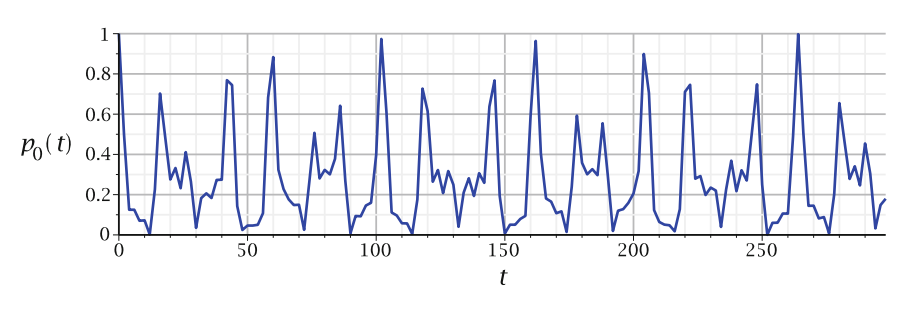
\includegraphics[width=0.8\textwidth]{Kap4/Quasiperiodyc10CyclePortugal.png}
\caption{Distribución del vértice $v=0$ en un 10-ciclo. \textit{Hay infinito número de tiempos en que el estado cuántico está cerca al estado inicial, presentando una estructura repetitiva en las escalas de tiempo.} \cite{portugal2013quantum}}
\end{figure}

La distribución después de muchos pasos depende de la estado inicial. Consideramos la distribución límite como la distribución uniforme sobre las distribuciones de probabilidad para cada estado inicial posible.

\subsubsection*{Gráfica 2D finita}
Una red 2D con condiciones de frontera periódicas corresponde a un \textit{toro}. Si la red tiene $N$ vértices, y sus lados $\sqrt{N}$, los estados en el modelo de moneda son $\{\ket{d,s}\otimes\ket{x,y}d,s=0,1,x,y=0,\dots \sqrt{N}-1\}$ en donde los estados de las monedas $\ket{d,s}$ están en $\mathcal{H}^2\otimes \mathcal{H}^2$, y son tales que $d$ designa el eje de movimiento: $d=0$ sobre el eje $x$, y $d=1$ sobre $y$, y $s$ la dirección, si $s=0$ hacia los negativos, $s=1$ hacia los positivos. Los estados de posición están en  $\mathcal{H}^{\sqrt{N}} \otimes   \mathcal{H}^{\sqrt{N}}$. La evolución dada por $\hat{U}=\hat{S}\hat{C}$. Un desarrollo similar al del anexo \ref{Anexo:SolucionLinea} lleva a la solución en cualquier tiempo:
%\begin{equation}
%    \hat{S}\ket{d,s}\ket{x,y}\xrightarrow{}\ket{d,s}\ket{x+(-1)^{\delta_{0,s}},y+(-1)^{\delta_{1,s}}}
%\end{equation}{}
\begin{equation}
    \ket{\psi(t)}=\dfrac{1}{\sqrt{N}}\ket{D}\ket{D}+\dfrac{1}{\sqrt{2N}}\sum_{\begin{array}{c} k,l=0\\ (k,l)\neq(0,0) \end{array}}^{\sqrt{N}-1} (e^{i\theta_klt}\ket{\nu_{kl}^{\theta}}+e^{-i\theta_klt}\ket{\nu_{kl}^{-\theta}})
\end{equation}
donde los autovalores y autovectores son 
\begin{equation}{}
\theta_{kl}=\frac{1}{2}(\cos{\dfrac{2\pi k}{\sqrt{N}}}+\cos{\dfrac{2\pi l}{\sqrt{N}}})\qquad\;\qquad
    \ket{\nu_{kl}^{\pm\theta}}=\dfrac{i}{2\sqrt{2}\sin{\theta_{kl}}}
      \left(
    \begin{array}{c}
        e^{i\theta_{kl}}-\omega^k   \\
        e^{-i\theta_{kl}}-\omega^{-k}\\
        e^{-i\theta_{kl}}-\omega^{l}\\
        e^{-i\theta_{kl}}-\omega^{-l}
    \end{array}
    \right),
\end{equation}

\subsubsection*{Hipercubo}
El hipercubo en $d$ dimensiones tiene $2^n$ vértices que son cadenas de $n$-bits, por ejemplo, $010011$ pertenece al $6$-hipercubo. El peso de Hamming de un vértice es el número de $1$'s en su nombre. Dos vértices están conectados si la distancia de Hamming es $1$.

\cite{marquezino2008mixing}\\

[17 en Kempe] La caminata cuántica sobre el hipercubo no se mezcla bajo ningún modelo, y eso parece una desventaja sobre el caso clásico, que, recordemos, siempre alcanza una distribución uniforme. Por otra parte, el tiempo de arribo \textit{hitting time} logra una mejora exponencial sobre el caso clásico. 

\subsubsection*{Gráfica de árboles ligados}

\begin{figure}[ht]
\centering
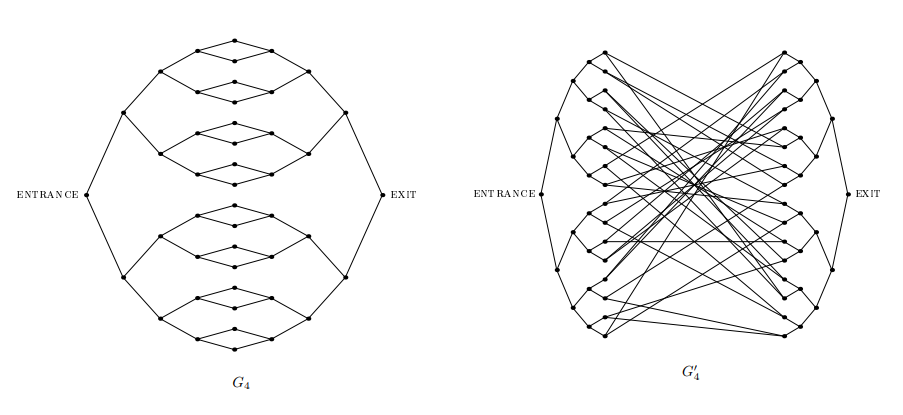
\includegraphics[width=1\textwidth]{Kap4/GluedTreesChilds.png}
\caption{La distancia de la mitad no es importante, sirve para esclarecer la imagen.  $G_n$ es más sencilla que $G_n'$. 
\label{gr:Gn}\cite{childs2003exponential}}
\end{figure}
\cite{childs2003exponential} usaron el modelo continuo para la caminata con el fin de analizar la propagación de una partícula en la gráfica de árboles ligados con profundidad $n$ (número de ramificaciones en cada lado), $G_n$. Compararon el \textit{hitting time} para alcanzar el vértice EXIT partiendo desde ENTRANCE obteniendo una ventaja exponencial con la caminata cuántica.

\begin{figure}[ht]
\centering
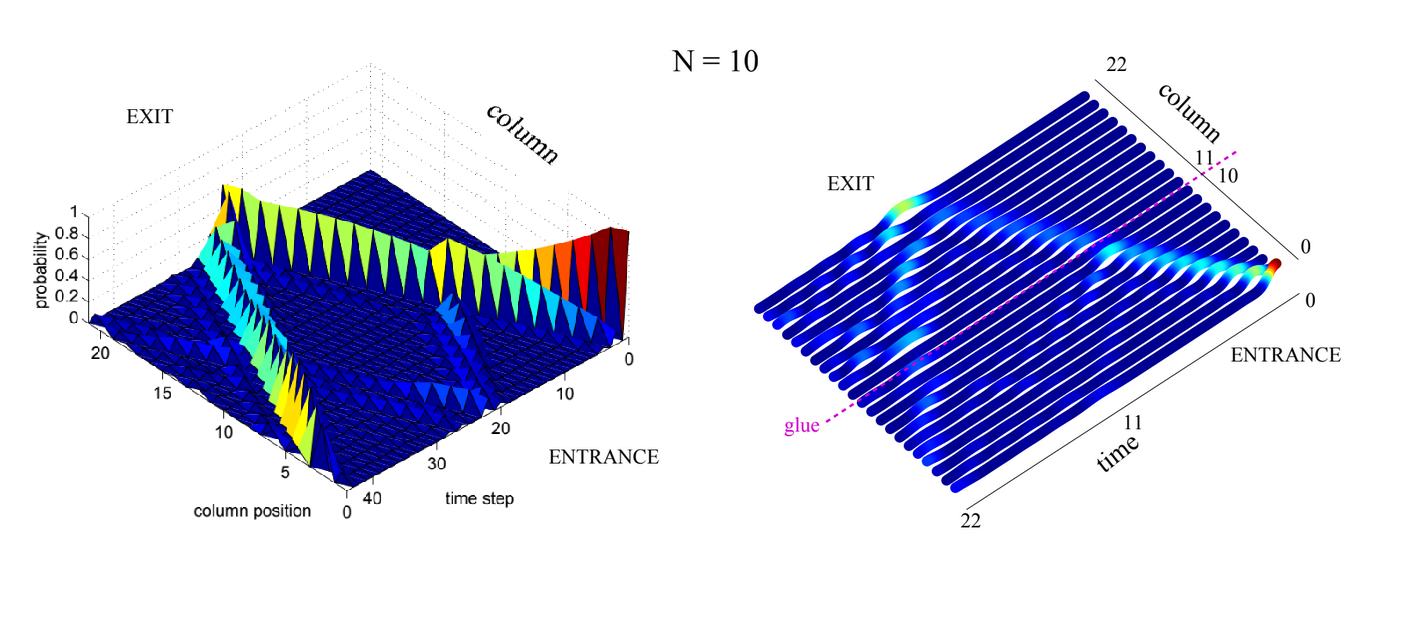
\includegraphics[width=1\textwidth]{Kap4/GluedTreesCarneiro.png}
\caption{Caminata de tiempo discreto y tiempo continuo sobre $G_4'$, para $N=10$. \cite{carneiro2005entanglement}}
\end{figure}

\begin{equation*}
    \ket{\text{col}\,j}=\dfrac{1}{\sqrt{N_j}}\sum_{v\,\in \, \text{column}\,j} \ket{v},
\end{equation*}{}
donde
\begin{equation}{}
    N_j=
    \left\{
    \begin{array}{ll}
    2^j & 0\leq j\leq n\\
    2^{2n+1-j} & n+1\leq j \leq 2n+1
    \end{array}
    \right.
\end{equation*}{}
\begin{equation*}
    \bra{\text{col}\,j}H\ket{\text{col}\,(j+1)}=
    \left\{
    \begin{array}{ll}
    \sqrt{2}\gamma     & 0\leq j\leq n-1\,,\,\,\,n+1\leq j\leq 2n  \\
    2\gamma     & j=n 
    \end{array}{}
    \right.
\end{equation*}{}

\begin{equation*}
    \braket{j|p}=\dfrac{1}{\sqrt{2\pi}}e^{ipj},\,\,\,\,\,\,-\pi\leq p\leq\pi
\end{equation*}{}
having energies $E_p=2\cos p$
\begin{align*}
    G(j,k,t)&=\bra{k}e^{-i\hat{H}t}\ket{j}\\
    &=\dfrac{1}{2\pi}\int_{-\pi}^{\pi}dp e^{ip(k-j)-2it\cos p}\\
    &=(-i)^{k-j}J_{k-j}(2t), \,\,\,\,\,\, -\infty < j,k < \infty
\end{align*}{}

\begin{align}
    J_\nu(\nu/\cosh{\zeta})
\end{align}{}

La probabilidad de estar en la raíz derecha habiendo partido de la raíz izquierda es:
\begin{equation}
    \Vec{\pi}\geq \frac{1}{2n+1},
\end{equation}
por su parte en el caso clásico:
\begin{align}
    \pi_b&=\lim_{t\xrightarrow{}\infty} p_b(t),\\
    \pi_b&=(2^{n+1}+2^n-2)^{-1}
\end{align}
\cite{childs2002example}

\subsubsection{Árbol de hexágonos}
En este caso no presentamos desarrollos analíticos sino los resultados de implementaciones experimentales. 

\begin{figure}[ht]
\centering
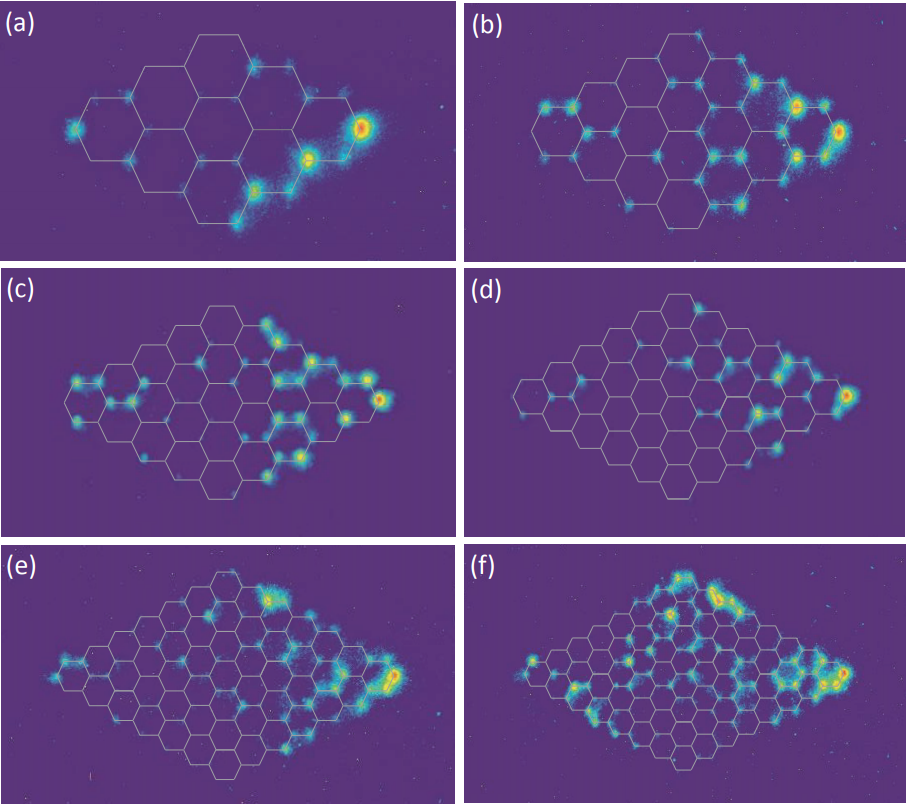
\includegraphics[width=0.7\textwidth]{Kap5/HexagonWalkTang2018.png}
\caption{Experimental }
\end{figure}


%\begin{figure}[ht]
%\caption{addfad}
%\centering
%\includegraphics[width=0.5\textwidth]{.png}
%\end{figure}
